\section{第六章 Harnessing
Engine：LLM约束引擎设计}\label{ux7b2cux516dux7ae0-harnessing-enginellmux7ea6ux675fux5f15ux64ceux8bbeux8ba1}

\subsection{6.1 Harnessing
Engine概念与架构}\label{harnessing-engineux6982ux5ff5ux4e0eux67b6ux6784}

\subsubsection{6.1.1
问题定义：LLM在硬件设计中的失败模式}\label{ux95eeux9898ux5b9aux4e49llmux5728ux786cux4ef6ux8bbeux8ba1ux4e2dux7684ux5931ux8d25ux6a21ux5f0f}

大语言模型在代码生成任务中展现出令人期待的能力，但同时暴露出若干系统性失败模式。在硬件设计自动化这一高精度、强约束的应用场景中，这些失败模式尤为突出，且具有跨设计对象的共性------无论目标是密码学模块、信号处理
IP 核还是总线控制器，LLM 均可能产生以下五类失败：

\textbf{失败模式一：幻觉端口/信号}。LLM在生成Verilog代码时，可能凭借训练数据中的统计模式''自行发明''实际不存在的端口（如将\texttt{key\_in}改写为\texttt{key\_data}），或在例化子模块时连接错误的端口名称。由于Verilog对未声明信号有时会静默警告而非报错，这类错误可能通过编译但在仿真阶段才暴露。

\textbf{失败模式二：语法错误}。LLM生成的Verilog代码有时包含非法语法结构，如在\texttt{always}块中混用阻塞/非阻塞赋值、在组合逻辑中使用时序敏感列表错误、参数化语法不兼容等。这类错误通常在L0编译门控阶段即可捕获，但若Agent仅修改部分代码而引入新的语法问题，则可能形成''修复一处、引入两处''的循环。

\textbf{失败模式三：Scope
drift（范围漂移）}。Agent在修复单个模块问题时，可能''顺手''修改了其他模块的接口定义或共享头文件，破坏模块间的已冻结接口契约。这类问题在单模块测试中不可见，只有在集成阶段才会暴露。

\textbf{失败模式四：过度修改}。修复Agent面对一个编译错误时，可能大幅重写整个模块而非进行最小化修复，将原本正确的逻辑也一并破坏。这种''推倒重来''模式缺乏收敛保证，可能导致验证状态在REPAIRING和L0\_FAIL之间无限循环。

\textbf{失败模式五：格式错误}。LLM可能输出Markdown代码块包裹的Verilog代码、在RTL文件中夹杂自然语言解释、或将完整JSON文件内容逐字输出到对话中，破坏文件格式和上下文效率。

\subsubsection{6.1.2 Harnessing
Engine设计理念}\label{harnessing-engineux8bbeux8ba1ux7406ux5ff5}

针对上述失败模式，本文提出''Harnessing
Engine''（驾驭引擎）概念，作为一种通用的 LLM
行为约束框架模式。其核心设计理念是：\textbf{不依赖 LLM
自律，通过结构化的外部约束从六个层面系统性地驾驭 LLM 行为}。Harnessing
Engine
的六层架构（Skill/Prompt/Memory/Hooks/MCP/SlashCommand）是领域无关的约束模式------每一层的约束机制均可通过替换领域内容适配不同的硬件设计目标，甚至扩展到软件工程等其他
LLM 应用场景。

``Harnessing''（驾驭）一词的选择具有深刻的工程意涵：驾驭不是压制，而是通过设计良好的约束结构，引导LLM的能力在期望的范围内发挥作用。如同马具（harness）不限制马的力量，而是引导其方向，Harnessing
Engine不试图消除LLM的创造性，而是通过六层约束确保这种创造性不会越出工程规约的边界。

Harnessing Engine的六层约束从架构上形成了一个完整的防御体系：

\begin{figure}
\centering
\pandocbounded{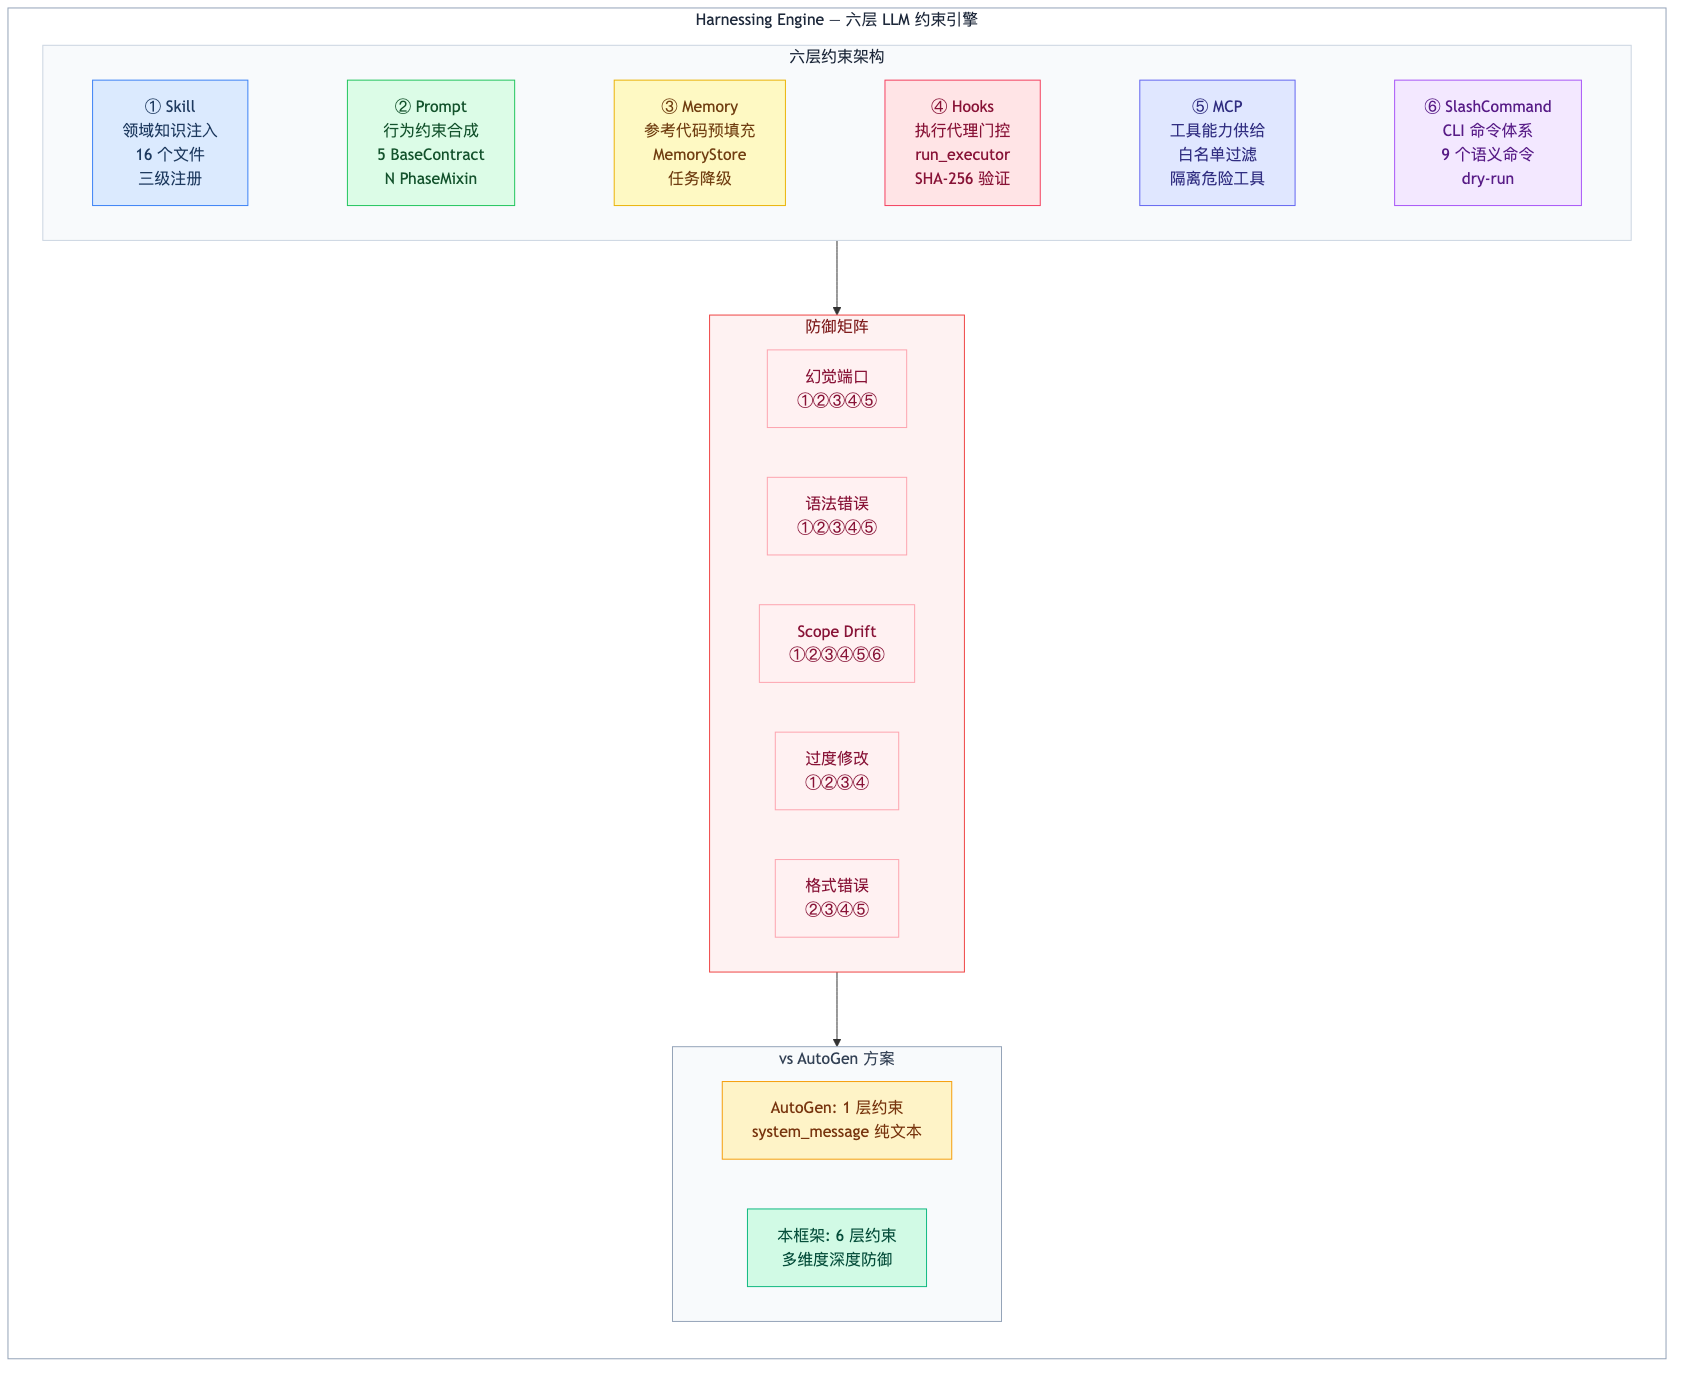
\includegraphics[keepaspectratio,alt={图6-1: Harnessing Engine六层约束架构总览}]{../fpga_flow/diagrams/16_harnessing_engine.png}}
\caption{图6-1: Harnessing Engine六层约束架构总览}
\end{figure}

\begin{figure}
\centering
\pandocbounded{
\includegraphics[keepaspectratio,alt={图6-2: Prompt合成流程}]{../fpga_flow/diagrams/10_prompt_composition.png}}
\caption{图6-2: Prompt合成流程}
\end{figure}

六层约束的分工如下表所示：

{[}表6-1: LLM失败模式-约束层级防御矩阵（详见6.8节）{]}

\begin{center}\rule{0.5\linewidth}{0.5pt}\end{center}

\subsection{6.2
Skill层：领域知识注入}\label{skillux5c42ux9886ux57dfux77e5ux8bc6ux6ce8ux5165}

\subsubsection{6.2.1
三级Skill注册体系}\label{ux4e09ux7ea7skillux6ce8ux518cux4f53ux7cfb}

Skill
层的三级注册体系（运行时/内存/文档）是一种通用的领域知识管理架构。运行时
Skill 注入运行时约束，内存 Skill 提供参考代码，文档 Skill
辅助离线合成。这一三级架构可直接复用于其他硬件设计------替换 Skill
文件内容即可适配新的设计领域。在 AES-128 验证案例中，16 个 Skill
文件按以下方式实例化：

本框架构建了由16个Skill文件组成的三级注册体系，通过\texttt{skill\_refs.py}统一管理。三级注册体系的分工严格区分了运行时注入与离线参考的职责：

\textbf{运行时Skill（Runtime
Skills，5个）}：通过\texttt{get\_runtime\_skill\_refs()}（\texttt{fpga\_flow/skill\_refs.py:22-51}）获取，直接注入到Agent的系统提示词中，在运行时作为硬约束约束Agent行为：

{\def\LTcaptype{none} % do not increment counter
\begin{longtable}[]{@{}
  >{\raggedright\arraybackslash}p{(\linewidth - 4\tabcolsep) * \real{0.4286}}
  >{\raggedright\arraybackslash}p{(\linewidth - 4\tabcolsep) * \real{0.2857}}
  >{\raggedright\arraybackslash}p{(\linewidth - 4\tabcolsep) * \real{0.2857}}@{}}
\toprule\noalign{}
\begin{minipage}[b]{\linewidth}\raggedright
Skill键
\end{minipage} & \begin{minipage}[b]{\linewidth}\raggedright
名称
\end{minipage} & \begin{minipage}[b]{\linewidth}\raggedright
用途
\end{minipage} \\
\midrule\noalign{}
\endhead
\bottomrule\noalign{}
\endlastfoot
\texttt{aes\_verilator\_profile} & aes-verilator-profile &
AES节点分类、向量、Checkpoint、L2约定 \\
\texttt{aes\_module\_patterns} & aes-module-patterns &
S-box、密钥扩展、轮变换、顶层集成的参考模式 \\
\texttt{aes\_tb\_contracts} & aes-tb-contracts & 自检C++
Testbench契约、向量和Checkpoint语义 \\
\texttt{aes\_repair\_heuristics} & aes-repair-heuristics &
编译/Checkpoint/延迟/握手失败的修复启发式规则 \\
\texttt{openhands\_sdk\_subagent\_delegation} &
openhands-sdk-subagent-delegation &
子Agent注册、spawn、委派和任务边界规则 \\
\end{longtable}
}

\textbf{内存Skill（Memory
Skills，5个）}：通过\texttt{get\_memory\_skill\_refs()}（\texttt{fpga\_flow/skill\_refs.py:54-83}）获取，由\texttt{MemoryStore}管理，包含验证通过的AES参考RTL代码，用于工作区预填充：

{\def\LTcaptype{none} % do not increment counter
\begin{longtable}[]{@{}
  >{\raggedright\arraybackslash}p{(\linewidth - 4\tabcolsep) * \real{0.3750}}
  >{\raggedright\arraybackslash}p{(\linewidth - 4\tabcolsep) * \real{0.3750}}
  >{\raggedright\arraybackslash}p{(\linewidth - 4\tabcolsep) * \real{0.2500}}@{}}
\toprule\noalign{}
\begin{minipage}[b]{\linewidth}\raggedright
Skill键
\end{minipage} & \begin{minipage}[b]{\linewidth}\raggedright
对应模块
\end{minipage} & \begin{minipage}[b]{\linewidth}\raggedright
内容
\end{minipage} \\
\midrule\noalign{}
\endhead
\bottomrule\noalign{}
\endlastfoot
\texttt{aes\_memory\_sbox} & aes\_sbox & 验证通过的S-box
RTL+TB参考实现 \\
\texttt{aes\_memory\_key\_schedule} & aes\_key\_schedule\_128 &
验证通过的密钥扩展RTL+TB参考实现 \\
\texttt{aes\_memory\_round\_transform} & aes\_round\_transform &
验证通过的轮变换RTL+TB参考实现 \\
\texttt{aes\_memory\_encrypt\_core} & aes128\_encrypt\_core &
验证通过的顶层加密核RTL+TB参考实现 \\
\texttt{aes\_memory\_shared} & 公共 & aes\_sbox\_lut.vh +
aes\_tb\_common.hpp上下文 \\
\end{longtable}
}

\textbf{文档Skill（Documentation
Skills，6个）}：通过\texttt{get\_documentation\_skill\_refs()}（\texttt{fpga\_flow/skill\_refs.py:86-120}）获取，供\texttt{synthesis.py}中的\texttt{ModuleDesignBrief}生成使用，不注入Agent运行时提示词。

{[}表6-2: 16个Skill文件分类表（名称、类型、用途）{]}

\subsubsection{6.2.2
Skill分组与按角色注入}\label{skillux5206ux7ec4ux4e0eux6309ux89d2ux8272ux6ce8ux5165}

Skill按Agent角色分组，实现精准注入。\texttt{WORKER\_FPGA\_CORE\_SKILL\_KEYS}（\texttt{fpga\_flow/skill\_refs.py:158-163}）包含3个核心Worker技能；\texttt{REPAIR\_CORE\_SKILL\_KEYS}仅包含\texttt{aes\_repair\_heuristics}；\texttt{ORCHESTRATOR\_CORE\_SKILL\_KEYS}仅包含\texttt{aes\_verilator\_profile}。

\texttt{select\_worker\_skill\_keys(active\_mode)}函数根据当前工作模式动态选择技能子集：generate模式使用\texttt{WORKER\_FPGA\_CORE\_SKILL\_KEYS}，repair模式使用\texttt{REPAIR\_CORE\_SKILL\_KEYS}，l2\_execute模式使用\texttt{L2\_WORKER\_SKILL\_KEYS}（仅\texttt{aes\_verilator\_profile}）。这一按模式精准注入的设计减少了提示词的冗余信息，降低了LLM''混淆技能''的可能性。

\subsubsection{6.2.3
SKILLS\_AS\_AUTHORITY\_CONTRACT}\label{skills_as_authority_contract}

\texttt{SKILLS\_AS\_AUTHORITY\_CONTRACT}（\texttt{fpga\_flow/prompt\_contracts.py:72-77}）是Skill层的元约束：

\begin{verbatim}
Repository skills are the authority for FPGA, Verilator, and SDK policy;
do not paraphrase or restate them.
\end{verbatim}

这一约束明确告知Agent：Skill文件是工程策略的权威来源，Agent不得根据自身训练数据''推断''或''改写''技能内容。与AutoGen方案的对比：该方案仅有\texttt{system\_message}中的纯文本指令，无结构化技能体系，Agent可能基于通用训练数据''自行推断''HDL设计规则，而这些推断与项目规约可能存在偏差。

\begin{center}\rule{0.5\linewidth}{0.5pt}\end{center}

\subsection{6.3
Prompt层：行为约束合成}\label{promptux5c42ux884cux4e3aux7ea6ux675fux5408ux6210}

\subsubsection{6.3.1
可组合Prompt架构}\label{ux53efux7ec4ux5408promptux67b6ux6784}

可组合 Prompt 架构（BaseContract + PhaseMixin +
InstancePayload）是一种领域无关的提示词工程模式。BaseContract
定义不可覆盖的硬约束，PhaseMixin 提供阶段适配的补充约束，InstancePayload
注入任务具体参数。这一组合机制使得框架能够为不同设计对象的不同执行阶段精确定制
Agent 行为约束。

本框架的提示词不是单一的静态字符串，而是通过\texttt{compose\_prompt()}函数（\texttt{fpga\_flow/prompt\_contracts.py:32-49}）将四层组件动态组合而成：

\begin{Shaded}
\begin{Highlighting}[]
\KeywordTok{def}\NormalTok{ compose\_prompt(}
\NormalTok{    role\_intro: }\BuiltInTok{str}\NormalTok{,}
    \OperatorTok{*}\NormalTok{,}
\NormalTok{    base\_contracts: Iterable[BaseContract],}
\NormalTok{    phase\_mixins: Iterable[PhaseMixin] }\OperatorTok{=}\NormalTok{ (),}
\NormalTok{    instance\_payload: InstancePayload }\OperatorTok{|} \VariableTok{None} \OperatorTok{=} \VariableTok{None}\NormalTok{,}
\NormalTok{    skill\_block: }\BuiltInTok{str} \OperatorTok{|} \VariableTok{None} \OperatorTok{=} \VariableTok{None}\NormalTok{,}
\NormalTok{) }\OperatorTok{{-}\textgreater{}} \BuiltInTok{str}\NormalTok{:}
\end{Highlighting}
\end{Shaded}

四层组件的职责划分如下：

\begin{figure}
\centering
\pandocbounded{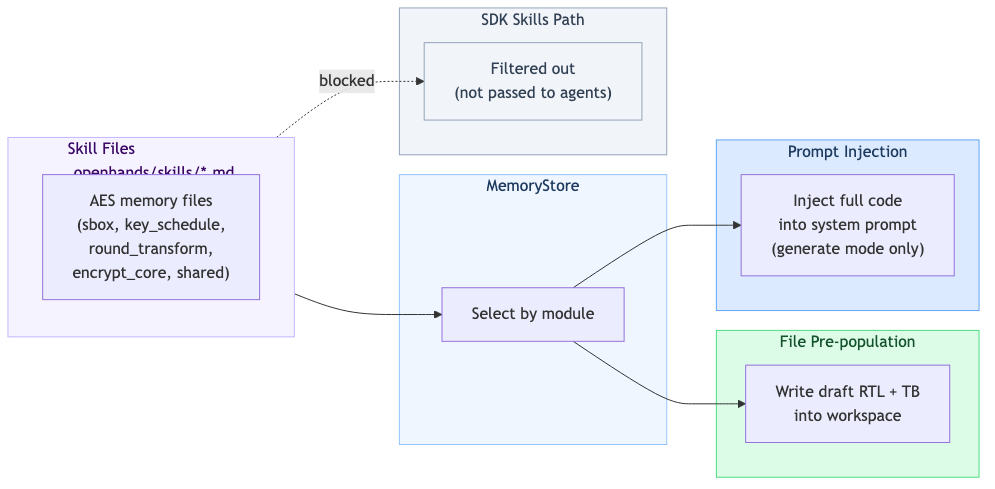
\includegraphics[keepaspectratio,alt={图6-3: Memory注入流程}]{../fpga_flow/diagrams/07_memory_injection.png}}
\caption{图6-3: Memory注入流程}
\end{figure}

\textbf{第一层：角色引言（role\_intro）}：声明Agent的身份和职责范围，如\texttt{You\ are\ the\ Module\ Worker\ SubAgent\ for\ aes\_sbox.}，确立了任务局部性。

\textbf{第二层：基础合约（BaseContract）}：硬约束集合，在所有工作模式下均有效，不可覆盖。5个核心BaseContract的约束维度各异：

{\def\LTcaptype{none} % do not increment counter
\begin{longtable}[]{@{}
  >{\raggedright\arraybackslash}p{(\linewidth - 4\tabcolsep) * \real{0.4000}}
  >{\raggedright\arraybackslash}p{(\linewidth - 4\tabcolsep) * \real{0.3000}}
  >{\raggedright\arraybackslash}p{(\linewidth - 4\tabcolsep) * \real{0.3000}}@{}}
\toprule\noalign{}
\begin{minipage}[b]{\linewidth}\raggedright
BaseContract
\end{minipage} & \begin{minipage}[b]{\linewidth}\raggedright
约束维度
\end{minipage} & \begin{minipage}[b]{\linewidth}\raggedright
核心条款
\end{minipage} \\
\midrule\noalign{}
\endhead
\bottomrule\noalign{}
\endlastfoot
AES\_SCOPE\_CONTRACT & 范围锁定 &
AES-128加密专用，encrypt-only，block-handshake \\
STRUCTURED\_IO\_CONTRACT & IO规范 &
以契约JSON为信息源，禁止cat完整大型JSON文件 \\
NO\_RAW\_VERILATOR\_CONTRACT & 工具隔离 &
禁止直接调用verilator\_compile或verilator\_simulate \\
FRAMEWORK\_OWNS\_PROGRESS\_CONTRACT & 控制权归属 &
框架而非Agent拥有批次推进和工作流完成权 \\
SKILLS\_AS\_AUTHORITY\_CONTRACT & 权威源 &
Skill文件是FPGA/Verilator/SDK策略的权威 \\
\end{longtable}
}

\textbf{第三层：阶段混入（PhaseMixin）}：针对当前执行阶段的补充约束，随工作模式动态切换。例如，\texttt{REPAIR\_PHASE\_ROUND\_1}要求''第一个工具调用必须是对primary\_target\_file的file\_editor
edit''，强制Agent先编辑后验证，防止无效的信息收集操作浪费修复轮次预算。

\textbf{第四层：实例负载（InstancePayload）}：当前任务的具体参数，如可写文件列表、Campaign参数、特殊行为注记等。

\subsubsection{6.3.2
PhaseMixin的阶段适配机制}\label{phasemixinux7684ux9636ux6bb5ux9002ux914dux673aux5236}

本框架在Prompt构建中对\textbf{非修复模式}与\textbf{修复模式}采用了完全不同的函数路径，这是有意为之的架构分离设计。

\textbf{非修复模式：\texttt{\_select\_phase\_mixins(active\_mode)}}（\texttt{fpga\_flow/prompts.py:91-114}）

该函数处理\texttt{generate}、\texttt{validate}、\texttt{l2\_execute}三种模式，由\texttt{build\_module\_worker\_prompt()}调用：

\begin{itemize}
\tightlist
\item
  \texttt{generate}模式：在基础混入（\texttt{WORKER\_LOCAL\_SCOPE}、\texttt{WORKER\_REQUEST\_AUTHORITY}、\texttt{RUN\_EXECUTOR\_PHASE}）之上加入\texttt{GENERATE\_PHASE}和\texttt{MEMORY\_CONSULTATION\_DIRECTIVE}
\item
  \texttt{validate}模式：在基础混入之上加入\texttt{VALIDATE\_PHASE}和\texttt{MEMORY\_CONSULTATION\_DIRECTIVE}（读多写少）
\item
  \texttt{l2\_execute}模式：在基础混入之上加入\texttt{L2\_PHASE}（禁止RTL/TB编辑）
\end{itemize}

\textbf{关键约束}：若\texttt{active\_mode=\textquotesingle{}repair\textquotesingle{}}传入\texttt{\_select\_phase\_mixins()}，函数会\textbf{抛出\texttt{ValueError}}（\texttt{fpga\_flow/prompts.py:97-101}），明确禁止通过此路径构建修复Prompt：

\begin{Shaded}
\begin{Highlighting}[]
\ControlFlowTok{elif}\NormalTok{ active\_mode }\OperatorTok{==} \StringTok{\textquotesingle{}repair\textquotesingle{}}\NormalTok{:}
    \ControlFlowTok{raise} \PreprocessorTok{ValueError}\NormalTok{(}
        \StringTok{\textquotesingle{}Use build\_repair\_worker\_prompt() for repair mode, \textquotesingle{}}
        \StringTok{"not build\_module\_worker\_prompt(active\_mode=\textquotesingle{}repair\textquotesingle{})"}
\NormalTok{    )}
\end{Highlighting}
\end{Shaded}

\textbf{修复模式：\texttt{build\_repair\_worker\_prompt()}}（\texttt{fpga\_flow/prompts.py:198-226}）

修复工作器使用完全独立的Prompt构建函数，不经过\texttt{\_select\_phase\_mixins()}。该函数根据修复轮次选择阶段混入：

\begin{itemize}
\tightlist
\item
  \texttt{repair\_round\ \textless{}=\ 1}：使用\texttt{REPAIR\_PHASE\_ROUND\_1}（编辑优先协议------第一个工具调用必须是对\texttt{primary\_target\_file}的文件编辑，基于\texttt{repair\_request.json}中已提供的文件摘录直接修复，无需重新读文件）
\item
  \texttt{repair\_round\ \textgreater{}\ 1}：使用\texttt{REPAIR\_PHASE\_ROUND\_2\_PLUS}（允许先查看当前文件状态------先前的编辑可能已改变文件内容，Agent需以磁盘状态为准进行针对性修复）
\end{itemize}

修复Prompt还固定注入\texttt{WORKER\_LOCAL\_SCOPE}和\texttt{REPAIR\_MEMORY\_DIRECTIVE}，但\textbf{不注入Memory
Block}------修复阶段的草稿文件可能已经过多轮修改，原始参考记忆已不反映当前磁盘状态。

这一架构分离的设计意图是：修复工作器与生成/验证工作器在行为约束上有本质差异，强制使用独立入口可以防止在修复路径中意外注入生成阶段的约束（如\texttt{MEMORY\_CONSULTATION\_DIRECTIVE}中对参考记忆的依赖），确保修复行为始终以当前磁盘状态为基准。

\subsubsection{6.3.3
典型反幻觉指令}\label{ux5178ux578bux53cdux5e7bux89c9ux6307ux4ee4}

Prompt层包含若干针对特定幻觉模式的反幻觉指令：

\begin{itemize}
\tightlist
\item
  \texttt{"Never\ cat\ whole\ large\ JSON\ files;\ use\ bounded\ reads\ only"}
  --- 防止Agent将整个工作区JSON文件内容输出到对话，导致上下文溢出
\item
  \texttt{"first\ tool\ call\ MUST\ be\ a\ file\_editor\ edit\ on\ primary\_target\_file"}
  --- 防止修复Agent在预算有限的情况下浪费调用次数在信息收集上
\item
  \texttt{"Do\ not\ change\ cross-module\ architecture,\ frozen\ interfaces,\ or\ integration\ policy"}
  --- 防止Scope drift
\item
  \texttt{"Do\ not\ broadly\ scan\ unrelated\ paths\ before\ consulting\ the\ task\ contract"}
  --- 防止Agent在任务开始时进行无边界的文件系统探索
\end{itemize}

\begin{center}\rule{0.5\linewidth}{0.5pt}\end{center}

\subsection{6.4
Memory层：验证代码预填充}\label{memoryux5c42ux9a8cux8bc1ux4ee3ux7801ux9884ux586bux5145}

\subsubsection{6.4.1
MemoryStore核心机制}\label{memorystoreux6838ux5fc3ux673aux5236}

Memory
层的核心机制------将验证通过的参考代码预填充到工作区------是一种通用的
LLM 任务降级策略。通过提供高质量参考实现，Agent
的任务从''从零生成正确代码''降级为''基于参考实现解决集成问题''，显著降低了出错概率。这一策略适用于任何拥有参考实现库的硬件设计领域。在
AES-128 验证案例中，\texttt{MemoryStore} 管理 4 个模块的参考 RTL 和
Testbench。

\texttt{MemoryStore}（\texttt{fpga\_flow/memory.py:57-174}）是AES参考内存检索的单一信息源，封装了从Skill文件中提取验证通过代码的完整逻辑。其核心注册表为\texttt{\_MEMORY\_REGISTRY}（\texttt{fpga\_flow/memory.py:18-23}）：

\begin{Shaded}
\begin{Highlighting}[]
\NormalTok{\_MEMORY\_REGISTRY: }\BuiltInTok{dict}\NormalTok{[}\BuiltInTok{str}\NormalTok{, }\BuiltInTok{str}\NormalTok{] }\OperatorTok{=}\NormalTok{ \{}
    \StringTok{\textquotesingle{}aes\_sbox\textquotesingle{}}\NormalTok{: }\StringTok{\textquotesingle{}aes\_memory\_sbox\textquotesingle{}}\NormalTok{,}
    \StringTok{\textquotesingle{}aes\_key\_schedule\_128\textquotesingle{}}\NormalTok{: }\StringTok{\textquotesingle{}aes\_memory\_key\_schedule\textquotesingle{}}\NormalTok{,}
    \StringTok{\textquotesingle{}aes\_round\_transform\textquotesingle{}}\NormalTok{: }\StringTok{\textquotesingle{}aes\_memory\_round\_transform\textquotesingle{}}\NormalTok{,}
    \StringTok{\textquotesingle{}aes128\_encrypt\_core\textquotesingle{}}\NormalTok{: }\StringTok{\textquotesingle{}aes\_memory\_encrypt\_core\textquotesingle{}}\NormalTok{,}
\NormalTok{\}}
\end{Highlighting}
\end{Shaded}

每个\texttt{module\_id}映射到对应的内存Skill键，Skill文件中包含经过Verilator验证的RTL
Verilog和C++
Testbench代码，通过Markdown代码块（\texttt{verilog\textasciigrave{}和}cpp\texttt{）标记。}\_extract\_code\_block()\texttt{函数（}fpga\_flow/memory.py:39-44`）使用正则表达式提取特定语言的代码块内容。

\subsubsection{6.4.2
两种使用模式}\label{ux4e24ux79cdux4f7fux7528ux6a21ux5f0f}

Memory层提供两种互补的使用模式：

\textbf{\texttt{populate\_workspace()}}（\texttt{fpga\_flow/memory.py:114-159}）：生成模式。将参考代码写入工作区\texttt{draft/rtl/\textless{}module\_id\textgreater{}.v}和\texttt{draft/tb/\textless{}module\_id\textgreater{}\_tb.cpp}文件。写入采用''仅在不存在时写入''的策略（\texttt{if\ not\ rtl\_path.exists():\ rtl\_path.write\_text(...)}），防止覆盖Agent已进行的修改。若内存提取失败（RTL或TB为None），则抛出\texttt{RuntimeError}，这是一个硬错误------框架不允许在无参考实现的情况下进入生成阶段。

\textbf{\texttt{build\_prompt\_block()}}（\texttt{fpga\_flow/memory.py:97-112}）：提示词注入模式。将参考代码以\texttt{===\ MEMORY:\ \textless{}name\textgreater{}\ ===}块的形式直接注入Agent系统提示词，使Agent在生成模式下能够''看到''参考实现：

\begin{verbatim}
=== MEMORY: aes-memory-sbox ===
[skill文件内容，含验证通过的Verilog和C++代码]
=== END MEMORY ===
\end{verbatim}

这一设计的核心洞察是：\textbf{将Agent的任务从''从零生成正确代码''降级为''基于参考实现解决集成问题''}。从零生成正确的AES
RTL代码需要LLM同时掌握AES算法、Verilog语法、Verilator兼容性规约和Checkpoint协议，任何一项理解偏差都会导致失败。而基于参考实现进行适应性修改，Agent只需关注当前任务的具体差异，显著降低了出错概率。

\subsubsection{6.4.3
MEMORY\_CONSULTATION\_DIRECTIVE与REPAIR\_MEMORY\_DIRECTIVE的区分}\label{memory_consultation_directiveux4e0erepair_memory_directiveux7684ux533aux5206}

两个Memory相关的PhaseMixin体现了不同阶段的内存使用策略：

\texttt{MEMORY\_CONSULTATION\_DIRECTIVE}（\texttt{fpga\_flow/prompt\_contracts.py:185-194}）用于generate/validate模式：

\begin{verbatim}
Your workspace draft files are pre-populated from verified AES reference memory.
The === MEMORY === blocks in your system prompt contain the same code that was
written to your draft files. The reference code passes all Verilator checkpoints.
You may reproduce it verbatim or adapt it.
\end{verbatim}

\texttt{REPAIR\_MEMORY\_DIRECTIVE}（\texttt{fpga\_flow/prompt\_contracts.py:196-204}）用于repair模式：

\begin{verbatim}
Your workspace draft files were originally pre-populated from verified AES reference
memory. The on-disk draft files are the current truth — they may have been modified
by prior repair rounds. Do not assume the original reference memory matches the
current file state. Always read the actual file before editing.
\end{verbatim}

这一区分防止了修复Agent基于''记忆中的参考实现''而非''磁盘上的当前状态''进行修复，避免了修复轮次之间状态不一致的问题。

\begin{center}\rule{0.5\linewidth}{0.5pt}\end{center}

\subsection{6.5
Hooks层：执行回调与门控}\label{hooksux5c42ux6267ux884cux56deux8c03ux4e0eux95e8ux63a7}

\subsubsection{6.5.1
run\_executor自定义工具}\label{run_executorux81eaux5b9aux4e49ux5de5ux5177}

run\_executor 自定义工具的代理模式适用于任何硬件设计------Agent
通过统一的工具接口触发编译和仿真，无需了解底层 EDA 工具的命令行细节。

\texttt{run\_executor}（\texttt{fpga\_flow/runtime/execution\_tools.py:30-147}）是本框架最重要的约束机制之一，也是Agent触发框架执行动作的唯一合法入口。其设计核心是：\textbf{通过单一受控工具替代多个原始工具，在Agent和底层EDA工具之间建立强制性的代理层}。

\texttt{run\_executor}的执行流程：

\begin{enumerate}
\def\labelenumi{\arabic{enumi}.}
\tightlist
\item
  Agent调用\texttt{run\_executor(request\_path=\textless{}task\_contract.json\textgreater{})}
\item
  \texttt{\_load\_task\_contract()}从路径读取并验证任务合约JSON（\texttt{DelegateBatchTask}
  Pydantic模型）
\item
  \texttt{\_infer\_executor\_kind()}根据任务模式推断执行器类型（GENERATE\_NODE、RUN\_NODE、RECORD\_REPAIR\_EDIT）
\item
  调度对应的执行器（\texttt{L0Executor}、\texttt{L1Executor}、\texttt{L2CampaignExecutor}、\texttt{IntegrationRegressionExecutor}）
\item
  返回\texttt{RunExecutorObservation}，包含执行状态、结果路径和下一步读取提示
\end{enumerate}

\subsubsection{6.5.2
RunExecutorObservation的引导性设计}\label{runexecutorobservationux7684ux5f15ux5bfcux6027ux8bbeux8ba1}

\texttt{RunExecutorObservation}（\texttt{fpga\_flow/runtime/execution\_tools.py:39-116}）不仅是执行结果的载体，还是Agent下一步行为的引导者。\texttt{next\_read\_paths}字段明确告知Agent执行结束后应读取哪些文件；\texttt{next\_read\_hints}中的\texttt{NextReadHints}包含\texttt{action}（READ\_ARTIFACTS、EDIT\_PRIMARY\_TARGET、WAIT\_FOR\_NEXT\_BATCH、ESCALATE\_TO\_ORCHESTRATOR）和\texttt{reason}字段，将框架的判断意图以结构化方式传达给Agent。

这一设计的意义在于：Agent接收到\texttt{run\_executor}的返回值后，不需要根据自身判断决定下一步查看什么文件或采取什么行动，而是遵循框架通过\texttt{next\_read\_hints}提供的明确指示，大幅减少了Agent决策的不确定性。

\subsubsection{6.5.3
verify\_repair\_edit哈希验证}\label{verify_repair_editux54c8ux5e0cux9a8cux8bc1}

\texttt{verify\_repair\_edit()}（\texttt{fpga\_flow/generation.py:680-735}）是Hooks层的另一核心机制，用于机器化验证修复编辑的真实性。其验证逻辑包含两个独立条件：

\textbf{条件一：文件哈希变化验证}。框架在写入修复请求前记录\texttt{primary\_target\_file}的SHA256哈希值（存入\texttt{repair\_contract.edit\_verification{[}\textquotesingle{}baseline\_hashes\textquotesingle{}{]}}），修复后对比当前哈希。若哈希未变化，说明Agent声称已修复但实际未修改文件，验证失败并拒绝推进至重新验证阶段。

\textbf{条件二：必要Token存在验证}。\texttt{repair\_contract.must\_add\_tokens}列出修复后文件必须包含的token（如\texttt{CHECKPOINT\textbar{}CHK\_XXX\textbar{}PASS\textbar{}}），框架验证这些token确实出现在修改后的文件中。验证器还接受等价形式：若token以\texttt{CHECKPOINT\textbar{}}开头，则\texttt{emit\_checkpoint("CHK\_XXX",\ ...)}调用也被视为满足要求。

这一双重验证机制彻底消除了Agent''虚假声称修复成功''的可能性------没有真实的文件修改和必要代码的添加，框架不会进入重新验证阶段。

\subsubsection{6.5.4 Batch
Gate回调机制}\label{batch-gateux56deux8c03ux673aux5236}

框架通过文件系统轮询实现Batch
Gate，将文件系统作为Agent和框架之间的通信通道：Agent将执行结果写入工作区文件（如\texttt{validation\_summary.json}、\texttt{module\_run\_result.json}），框架的\texttt{run\_current\_batch\_until\_gate()}定期轮询这些文件，判断批次完成条件。当所有节点均有结果文件产生且状态满足门控条件时，框架结束当前批次，推进到下一状态。

\begin{center}\rule{0.5\linewidth}{0.5pt}\end{center}

\subsection{6.6
MCP层：工具能力供给}\label{mcpux5c42ux5de5ux5177ux80fdux529bux4f9bux7ed9}

\subsubsection{6.6.1 Model Context
Protocol的角色}\label{model-context-protocolux7684ux89d2ux8272}

MCP 工具过滤机制是通用的，可根据不同场景配置排除列表。

Model Context Protocol（MCP）是AI
Agent与外部工具之间的标准化通信协议。在本框架中，MCP承担着连接LLM
Agent与Verilator
EDA工具链的桥梁角色，将复杂的Verilator命令行接口封装为Agent可调用的结构化工具接口。

\begin{figure}
\centering
\pandocbounded{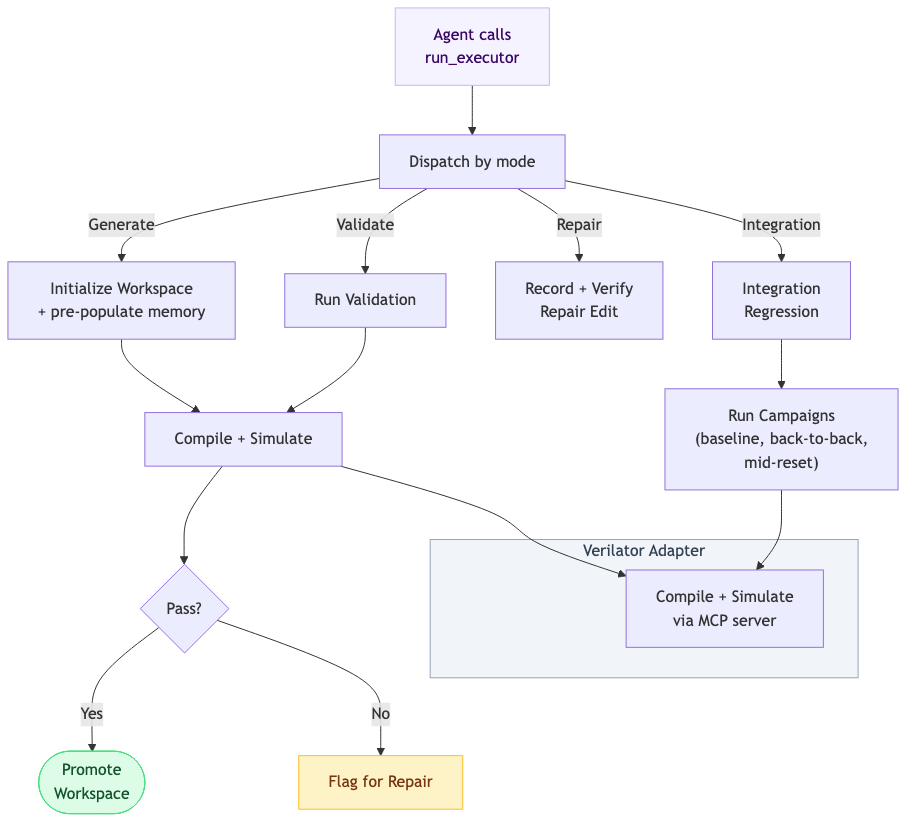
\includegraphics[keepaspectratio,alt={图6-4: 执行器调度流程}]{../fpga_flow/diagrams/08_executor_dispatch.png}}
\caption{图6-4: 执行器调度流程}
\end{figure}

\begin{figure}
\centering
\pandocbounded{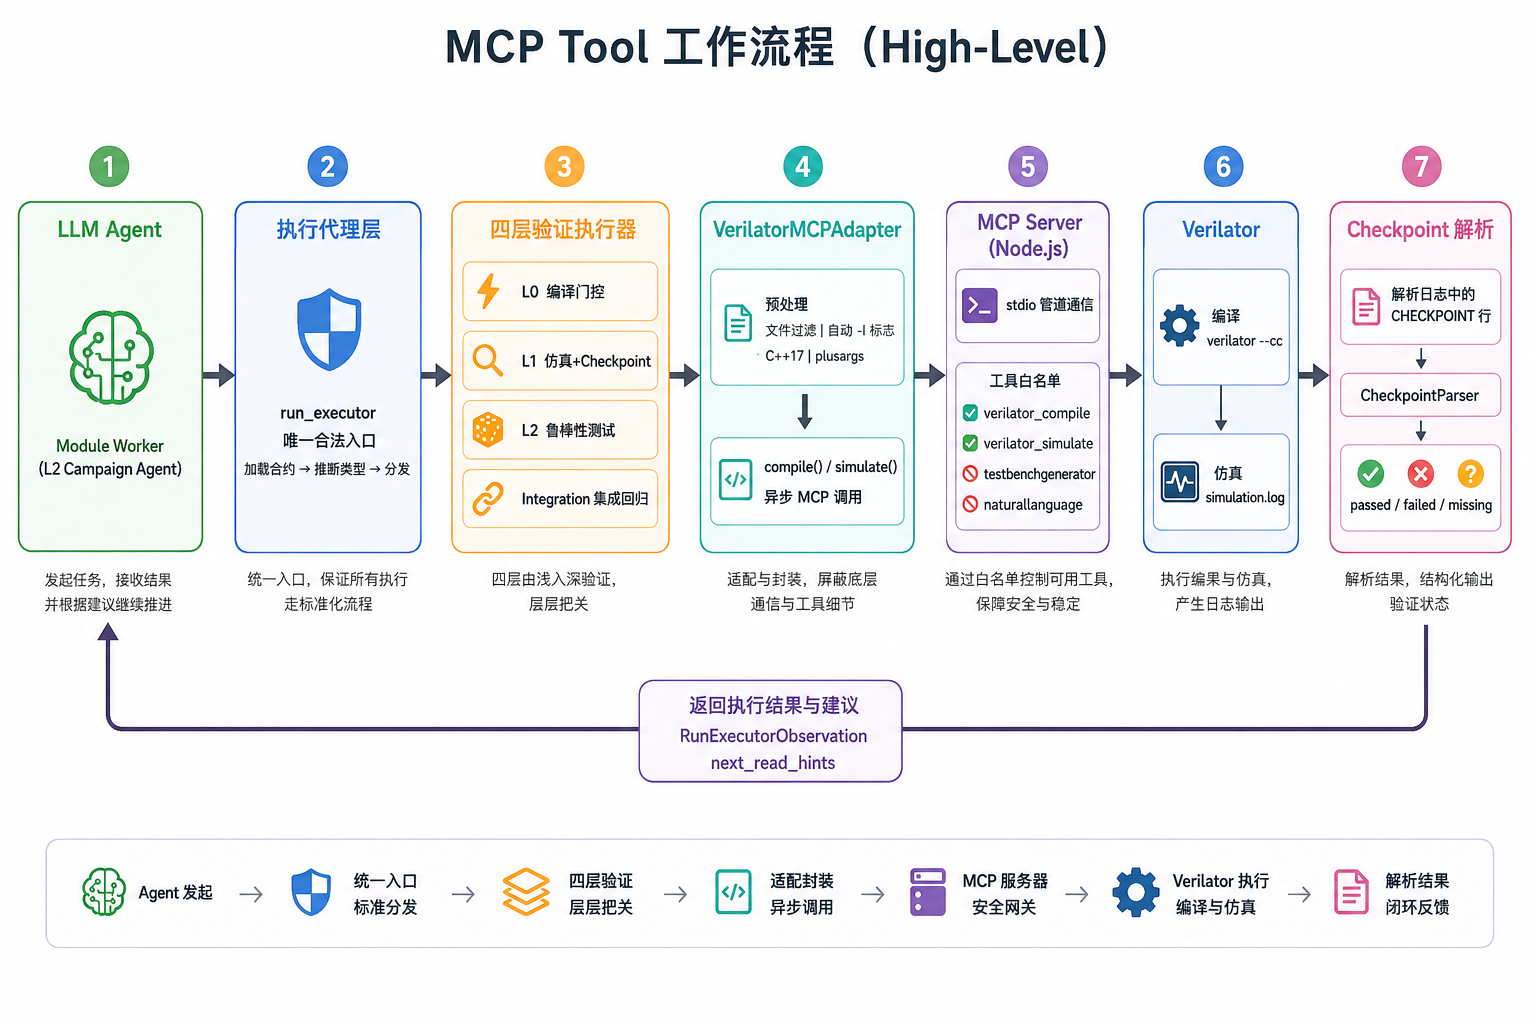
\includegraphics[keepaspectratio,alt={图6-5: MCP Verilator适配器架构}]{../fpga_flow/diagrams/15_mcp_verilator_adapter.png}}
\caption{图6-5: MCP Verilator适配器架构}
\end{figure}

\subsubsection{6.6.2
VerilatorMCPAdapter封装细节}\label{verilatormcpadapterux5c01ux88c5ux7ec6ux8282}

\texttt{VerilatorMCPAdapter}（\texttt{fpga\_flow/adapters/verilator.py:122-216}）封装了所有与Verilator
MCP服务器的通信细节，对上层执行器（L0/L1/L2/Integration
Executor）提供简洁的\texttt{compile()}和\texttt{simulate()}异步接口。其关键封装逻辑包括：

\textbf{输入文件过滤}：\texttt{\_filter\_verilator\_input\_files()}（\texttt{fpga\_flow/adapters/verilator.py:81-91}）过滤掉目录路径和非标准扩展名文件，只保留\texttt{.v}/\texttt{.sv}（Verilog源文件）和\texttt{.cpp}/\texttt{.cc}/\texttt{.cxx}（C++
Testbench）。这防止了Agent传入不合法文件路径导致Verilator报错。

\textbf{include标志自动生成}：\texttt{\_verilog\_include\_directories()}自动提取Verilog源文件的父目录，生成\texttt{-I/path/to/rtl}格式的include标志，确保\texttt{\textasciigrave{}include\ "aes\_sbox\_lut.vh"}等头文件引用能够正确解析。

\textbf{C++17标准自动添加}：当编译文件列表中包含C++源文件时，自动在\texttt{verilatorFlags}中添加\texttt{-CFLAGS\ -std=c++17}，无需Agent手动指定编译选项。

\textbf{plusargs传递}：\texttt{fpga\_flow\_package\_root}等运行时参数通过Verilator
plusargs机制传递给Testbench，Testbench通过\texttt{resolve\_path(argc,\ argv,\ requested,\ fallback)}函数读取，实现了向量文件的路径无关解析。

\subsubsection{6.6.3
MCP工具过滤：防止Agent绕过框架}\label{mcpux5de5ux5177ux8fc7ux6ee4ux9632ux6b62agentux7ed5ux8fc7ux6846ux67b6}

\texttt{build\_verilator\_stdio\_server()}（\texttt{fpga\_flow/adapters/verilator.py:43-74}）配置MCP服务器时，框架在更高层（\texttt{SdkAgentFactory}）过滤掉两个MCP工具：\texttt{verilator\_testbenchgenerator}和\texttt{verilator\_naturallanguage}。这一过滤的设计意图是：

\begin{itemize}
\tightlist
\item
  \textbf{禁用testbenchgenerator}：防止Agent绕过框架的C++自检Testbench体系，使用自动生成的Testbench（自动Testbench无法实现Checkpoint协议）
\item
  \textbf{禁用naturallanguage}：防止Agent以自然语言描述方式调用Verilator，绕过框架的结构化执行路径
\end{itemize}

这两个工具的禁用体现了MCP层的核心约束原则：Agent只能使用框架明确授权的工具子集，任何可能绕过约束体系的工具入口均被封闭。

\begin{center}\rule{0.5\linewidth}{0.5pt}\end{center}

\subsection{6.7
SlashCommand层：用户交互接口}\label{slashcommandux5c42ux7528ux6237ux4ea4ux4e92ux63a5ux53e3}

\subsubsection{6.7.1 CLI命令体系}\label{cliux547dux4ee4ux4f53ux7cfb}

CLI 命令体系的语义设计面向通用硬件设计验证流程。

\texttt{\_\_main\_\_.py}（\texttt{fpga\_flow/\_\_main\_\_.py}）实现了完整的CLI命令体系，每个命令对应一套完整的验证/执行语义：

\begin{Shaded}
\begin{Highlighting}[]
\ExtensionTok{python} \AttributeTok{{-}m}\NormalTok{ MultiAgent\_FPGA.fpga\_flow validate           }\CommentTok{\# 契约验证（无需API密钥）}
\ExtensionTok{python} \AttributeTok{{-}m}\NormalTok{ MultiAgent\_FPGA.fpga\_flow smoke{-}sdk           }\CommentTok{\# SDK烟测}
\ExtensionTok{python} \AttributeTok{{-}m}\NormalTok{ MultiAgent\_FPGA.fpga\_flow smoke{-}provider      }\CommentTok{\# DeepSeek API预检}
\ExtensionTok{python} \AttributeTok{{-}m}\NormalTok{ MultiAgent\_FPGA.fpga\_flow run{-}node }\OperatorTok{\textless{}}\NormalTok{module}\OperatorTok{\textgreater{}}   \CommentTok{\# 单节点L0+L1验证}
\ExtensionTok{python} \AttributeTok{{-}m}\NormalTok{ MultiAgent\_FPGA.fpga\_flow generate{-}node }\OperatorTok{\textless{}}\NormalTok{module}\OperatorTok{\textgreater{}}  \CommentTok{\# 工作区初始化+验证}
\ExtensionTok{python} \AttributeTok{{-}m}\NormalTok{ MultiAgent\_FPGA.fpga\_flow record{-}repair{-}edit }\OperatorTok{\textless{}}\NormalTok{module}\OperatorTok{\textgreater{}}  \CommentTok{\# 记录修复编辑}
\ExtensionTok{python} \AttributeTok{{-}m}\NormalTok{ MultiAgent\_FPGA.fpga\_flow run{-}integration     }\CommentTok{\# 集成回归测试}
\ExtensionTok{python} \AttributeTok{{-}m}\NormalTok{ MultiAgent\_FPGA.fpga\_flow run{-}aes{-}mvp         }\CommentTok{\# 全流程自主执行}
\ExtensionTok{python} \AttributeTok{{-}m}\NormalTok{ MultiAgent\_FPGA.fpga\_flow run{-}aes{-}mvp }\AttributeTok{{-}{-}dry{-}run}  \CommentTok{\# 干运行（仅规划，不执行）}
\end{Highlighting}
\end{Shaded}

\subsubsection{6.7.2
命令即合约的设计原则}\label{ux547dux4ee4ux5373ux5408ux7ea6ux7684ux8bbeux8ba1ux539fux5219}

每个CLI命令背后是完整的语义定义：\texttt{run-node}命令不仅调用执行器，还管理工作区状态（初始化、验证、修复预算检查）、生成报告文件、更新工作区记录；\texttt{record-repair-edit}命令先运行\texttt{verify\_repair\_edit()}验证修复真实性，再调用\texttt{write\_edit\_receipt()}写入编辑收据，为后续重新验证提供可追溯的审计链。

\texttt{-\/-dry-run}选项实现了规划与执行的分离：框架完成全部初始化（bootstrap、SpecIR/PlanDAG/Manifest合成、Policy验证），但仅输出将要执行的批次计划而不实际调用LLM
API，供用户在正式运行前检查执行策略。

\begin{center}\rule{0.5\linewidth}{0.5pt}\end{center}

\subsection{6.8
六层协同：约束覆盖矩阵}\label{ux516dux5c42ux534fux540cux7ea6ux675fux8986ux76d6ux77e9ux9635}

\subsubsection{6.8.1
LLM失败模式-约束层级防御矩阵}\label{llmux5931ux8d25ux6a21ux5f0f-ux7ea6ux675fux5c42ux7ea7ux9632ux5fa1ux77e9ux9635}

六层约束并非相互独立，而是形成了对LLM失败模式的多层防御体系。下表展示了每种失败模式由哪些约束层级防御：

{[}表6-3: LLM失败模式-约束层级防御矩阵{]}

{\def\LTcaptype{none} % do not increment counter
\begin{longtable}[]{@{}
  >{\raggedright\arraybackslash}p{(\linewidth - 12\tabcolsep) * \real{0.1429}}
  >{\raggedright\arraybackslash}p{(\linewidth - 12\tabcolsep) * \real{0.1270}}
  >{\raggedright\arraybackslash}p{(\linewidth - 12\tabcolsep) * \real{0.1429}}
  >{\raggedright\arraybackslash}p{(\linewidth - 12\tabcolsep) * \real{0.1429}}
  >{\raggedright\arraybackslash}p{(\linewidth - 12\tabcolsep) * \real{0.1270}}
  >{\raggedright\arraybackslash}p{(\linewidth - 12\tabcolsep) * \real{0.0952}}
  >{\raggedright\arraybackslash}p{(\linewidth - 12\tabcolsep) * \real{0.2222}}@{}}
\toprule\noalign{}
\begin{minipage}[b]{\linewidth}\raggedright
失败模式
\end{minipage} & \begin{minipage}[b]{\linewidth}\raggedright
Skill层
\end{minipage} & \begin{minipage}[b]{\linewidth}\raggedright
Prompt层
\end{minipage} & \begin{minipage}[b]{\linewidth}\raggedright
Memory层
\end{minipage} & \begin{minipage}[b]{\linewidth}\raggedright
Hooks层
\end{minipage} & \begin{minipage}[b]{\linewidth}\raggedright
MCP层
\end{minipage} & \begin{minipage}[b]{\linewidth}\raggedright
SlashCommand层
\end{minipage} \\
\midrule\noalign{}
\endhead
\bottomrule\noalign{}
\endlastfoot
\textbf{幻觉端口/信号} &
\texttt{aes\_module\_patterns}提供正确端口规范；\texttt{aes\_verilator\_profile}明确模块接口
&
\texttt{AES\_SCOPE\_CONTRACT}范围锁定；\texttt{WORKER\_REQUEST\_AUTHORITY}以合约为信息源
&
\texttt{populate\_workspace()}写入正确端口的参考RTL；\texttt{build\_prompt\_block()}内联参考实现
& L0编译门控捕获端口连接错误 & Verilator编译器严格验证端口声明 &
\texttt{validate}命令预检契约完整性 \\
\textbf{语法错误} &
\texttt{verilog\_verilator}提供Verilator合规Verilog规则；\texttt{aes\_tb\_contracts}提供合规TB模式
& \texttt{STRUCTURED\_IO\_CONTRACT}约束输出格式 &
参考实现本身是语法正确的Verilog代码 &
L0编译门控精确定位语法错误行；\texttt{RunExecutorObservation.next\_read\_hints}引导读取编译日志
& Verilator编译器是语法权威；自动添加\texttt{-CFLAGS\ -std=c++17} &
\texttt{run-node}命令明确L0失败含义 \\
\textbf{Scope drift} &
\texttt{openhands\_sdk\_subagent\_delegation}明确任务边界规则 &
\texttt{WORKER\_LOCAL\_SCOPE}限制可写范围；\texttt{ORCHESTRATOR\_ONLY\_CURRENT\_BATCH}限制批次范围
& \texttt{populate\_workspace()}只写入当前模块的draft目录 &
\texttt{run\_executor}只接受当前任务合约路径；\texttt{verify\_repair\_edit()}只验证primary\_target\_file
& 工具过滤禁用可能越界的工具 &
每个命令的workspace\_root参数限制操作范围 \\
\textbf{过度修改} &
\texttt{aes\_repair\_heuristics}提供最小化修复启发式规则 &
\texttt{REPAIR\_PHASE\_ROUND\_1}要求首次编辑仅针对primary\_target\_file；禁止secondary\_target\_files的预读
& \texttt{REPAIR\_MEMORY\_DIRECTIVE}要求以磁盘状态为准，不基于记忆重写 &
\texttt{verify\_repair\_edit()}双重验证（哈希+token）；修复预算限制（默认2次）
& --- & \texttt{record-repair-edit}命令强制显式编辑记录 \\
\textbf{格式错误} & --- & \texttt{STRUCTURED\_IO\_CONTRACT}：``Never cat
whole large JSON files''；以合约JSON为信息源 &
内存注入使用\texttt{===\ MEMORY\ ===}块而非原始文件内容 &
\texttt{RunExecutorObservation.to\_llm\_content}将执行结果序列化为结构化文本行
& MCP结果通过\texttt{\_extract\_text\_from\_result()}提取纯文本 &
CLI命令输出格式化JSON报告 \\
\end{longtable}
}

\subsubsection{6.8.2 一个Module
Worker的完整约束链路}\label{ux4e00ux4e2amodule-workerux7684ux5b8cux6574ux7ea6ux675fux94feux8def}

以\texttt{aes\_sbox}模块的generate阶段为例，展示六层约束的协同工作：

\begin{enumerate}
\def\labelenumi{\arabic{enumi}.}
\tightlist
\item
  \textbf{Skill层}：Agent系统提示词注入\texttt{aes\_verilator\_profile}、\texttt{aes\_module\_patterns}、\texttt{aes\_tb\_contracts}三个技能文件，Agent获取S-box模块的端口规范、Checkpoint协议规则和Testbench写法规范
\item
  \textbf{Prompt层}：\texttt{compose\_prompt()}组合\texttt{AES\_SCOPE\_CONTRACT}（范围锁定）、\texttt{NO\_RAW\_VERILATOR\_CONTRACT}（工具隔离）、\texttt{WORKER\_LOCAL\_SCOPE}（写作范围限于draft/）、\texttt{GENERATE\_PHASE}（工作区内生成）、\texttt{MEMORY\_CONSULTATION\_DIRECTIVE}（参考内存为权威）
\item
  \textbf{Memory层}：\texttt{MemoryStore.populate\_workspace(\textquotesingle{}aes\_sbox\textquotesingle{},\ workspace\_root)}将验证通过的S-box
  Verilog代码写入\texttt{draft/rtl/aes\_sbox.v}；\texttt{build\_prompt\_block(\textquotesingle{}aes\_sbox\textquotesingle{})}将参考代码内联到提示词中
\item
  \textbf{Hooks层}：Agent调用\texttt{run\_executor(request\_path=task\_contract.json)}
  → 框架执行L0+L1 →
  若L1通过，\texttt{RunExecutorObservation}返回\texttt{status:\ passed}；若L0失败，返回\texttt{next\_read\_hints:\ {[}action:\ EDIT\_PRIMARY\_TARGET,\ reason:\ "compile\ error"{]}}
\item
  \textbf{MCP层}：\texttt{VerilatorMCPAdapter}过滤输入文件，自动生成include标志，调用verilator-mcp的\texttt{verilator\_compile}和\texttt{verilator\_simulate}工具
\item
  \textbf{SlashCommand层}：整个过程通过\texttt{python\ -m\ MultiAgent\_FPGA.fpga\_flow\ run-node\ aes\_sbox}触发，命令封装了完整的工作区初始化、执行、报告生成语义
\end{enumerate}

\subsubsection{6.8.3
与AutoGen方案的约束密度对比}\label{ux4e0eautogenux65b9ux6848ux7684ux7ea6ux675fux5bc6ux5ea6ux5bf9ux6bd4}

本框架的六层约束体系在架构层面是通用的，其约束密度优势不依赖于 AES-128
这一特定设计对象。将框架适配到新的硬件设计时，需要替换的是 Skill
文件内容和 Memory 参考代码，而六层约束架构本身无需修改。

本框架采用六层约束驾驭LLM，而基于AutoGen的方案的约束主要集中于单一层（system\_message中的自然语言指令）。两种方案的约束密度对比：

{\def\LTcaptype{none} % do not increment counter
\begin{longtable}[]{@{}
  >{\raggedright\arraybackslash}p{(\linewidth - 4\tabcolsep) * \real{0.3462}}
  >{\raggedright\arraybackslash}p{(\linewidth - 4\tabcolsep) * \real{0.3077}}
  >{\raggedright\arraybackslash}p{(\linewidth - 4\tabcolsep) * \real{0.3462}}@{}}
\toprule\noalign{}
\begin{minipage}[b]{\linewidth}\raggedright
约束维度
\end{minipage} & \begin{minipage}[b]{\linewidth}\raggedright
本文方案
\end{minipage} & \begin{minipage}[b]{\linewidth}\raggedright
AutoGen方案
\end{minipage} \\
\midrule\noalign{}
\endhead
\bottomrule\noalign{}
\endlastfoot
领域知识注入 & 16个结构化Skill文件，按角色按阶段精准注入 &
system\_message中的纯文本描述 \\
提示词约束 & 5个BaseContract × N个PhaseMixin的可组合结构 &
单一system\_message \\
代码参考 & MemoryStore提供验证通过的参考RTL+TB & 无结构化代码参考 \\
执行验证 & \texttt{verify\_repair\_edit()}哈希验证；Batch Gate轮询 &
依赖Agent自报告 \\
工具隔离 & \texttt{run\_executor}单一入口；MCP工具白名单过滤 &
直接调用Vivado xsim \\
操作接口 & 9个语义明确的CLI命令 &
\texttt{human\_input\_mode="NEVER"}自运行 \\
\end{longtable}
}

这一对比表明，本框架的约束密度显著高于单层方案，在多个维度形成了对LLM失败模式的冗余防御。Harnessing
Engine的价值在于：即使某一层约束被LLM''绕过''（如Agent忽略了某个Prompt约束），其他层的约束仍能将行为控制在可接受范围内，形成了系统级的鲁棒性。

这种多层约束的设计哲学与系统工程中的''深度防御''原则一脉相承：单点约束在面对LLM的随机性和不可预测性时是脆弱的，而多层冗余约束则能在统计意义上保证系统行为的可靠性。
